\chapter{高速流场的数值计算及模拟}
在研究解决实际工程问题时,可以通过数值模拟地方法对所研究的流场进行模拟分析,能有效提高研究效率,流场的模拟主要通过对流体运动方程组实现离散的数值解,通过空间上的离散点的物理量来展现模拟结果。
目前的流体计算软件大多基于离散网格求解,当利用上一章提出的二方程模型对流场进行数值计算时,需要对控制方程进行离散,并且具体计算时首先需要初始化求解参数,然后通过迭代直至收敛,但是由于模型结构不同,初始参数也应该相应变化,实际流动问题的处理也较为复杂,如何确定定解条件成为了计算流体力学的一大难题,目前还没有形成一般性的理论\cite{yan2006},但可以根据已有的符合实际的经验参数作最大程度的近似计算。
\section{流场方程的计算}
实际求解流场的各项物理参数时主要可以基于有限体积法,将包含点的微元体积内的各项物理量看成与中心点一致,然后是由大量散点集合构成整个流场分布,对此可以将流场划分成大量的小网格,对流体运动方程离散求解,因此对于流场的正式计算,可以分成流场初始化条件设置即迭代开始条件及壁面等边界条件,然后通过离散方程进行迭代求解。
\subsection{求解条件的设置}
计算流体力学的定解条件分为流场初始条件和边界条件两个部分。初始条件需要根据具体的流动问题来设定,一般可以根据指定的初始状态计算相关来流参量,例如给定当前海拔高度,及海平面处大气温度,通过计算就能给出外界环境参量如温度、密度、大气压强等,并且给出飞行器飞行速度及机身与前进方向夹角,可以得到速度在$x,y,z$方向上的分量,而初始的湍流运输方程参量$k$及动能耗散率$\varepsilon$则可以参考已有经验参数进行设置,初始的内能可以根据能量边界方程确定。

边界条件的确定则对求解问题的精度及准确度影响较大,一般来说边界可分为壁面边界、出入口边界条件及远场边界,这三个边界条件决定了对流场结构进行模拟计算时的准确性,同时为了减少计算量,可以设置对称边界,对于对称性结构只计算一半,然后利用对称面进行复制即可,同时为了对计算域划分,可以设置链接界面,该界面仅仅用于计算识别功能,并不会对计算产生影响。

由于在计算模拟时,首先应该人为给出飞行器的飞行速度,远处大气密度、温度、压强等基本参量,而当前大气的压力温度密度等都可以借由所处位置距离海平面高度计算得知,大气中任意点的压力 $p$,密度$\rho$及温度$T$满足状态方程\eqref{eq:zhuangtai},并且处于力学平衡的大气应满足公式\eqref{eq:pingheng}、\eqref{eq:pzgongshi}:
\begin{align}
p=\rho RT/m\label{eq:zhuangtai}\\
dp=-\rho gdz\label{eq:pingheng}\\
\frac{dp}{p}=\frac{mg}{RT}dz\label{eq:pzgongshi}
\end{align}
式中,$m$为混合气体平均分子质量,$z$为海拔高度,$g$为关于$z$的重力加速度。

通过上述状态方程等构成的方程组,可以看出,只要给出当前海拔高度,就能够明确得到该位置的大气压值以及空气密度,在10km以下高度每提高1km,温度大约会下降6.5K,表\ref{tab:haibacanshu}给出了$0\sim6$km的对流层大气参数,事实上当高度大于10km进入平流层后,随着高度的增加大气温度基本会保持不变,密度、压强则会持续下降。
\begin{table}[tbhp]
\centering
\caption{密度压力温度随海拔的分布}
\label{tab:haibacanshu}
\begin{tabular}{|c|c|c|c|}
\hline
$z/\text{km}$&$\rho/(\text{kg}/\text{m}^3)$&$p/\text{Pa}$&$T/\text{K}$\\\hline
$0$&$1.2250$&$1.101325\times10^5$&$288.150$\\\hline
$1$&$1.1117$&$8.9876\times10^4$&$281.651$\\\hline
$2$&$1.0066$&$7.9501\times10^4$&$275.154$\\\hline
$3$&$9.0925\times10^{-1}$&$7.0121\times10^4$&$268.659$\\\hline
$4$&$8.1935\times10^{-1}$&$6.1660\times10^4$&$262.166$\\\hline
$5$&$7.3643\times10^{-1}$&$5.4048\times10^4$&$255.676$\\\hline
$6$&$6.6011\times10^{-1}$&$4.7217\times10^4$&$249.187$\\\hline
\end{tabular}
\end{table}

除了远场的密度、大气压、温度等初始流场参数,初始条件还需要设置初始内能以及在进行模拟时选定初始的$k,\varepsilon$的值或者$k-\varepsilon$,这可以根据一般的经验参照Menter\cite{menter1994}的建议进行取值,而无穷远处来流的初始内能一般满足方程\eqref{eq:lailiuneineng}。
\begin{equation}
e=\frac{1}{\gamma-1}\cdot\frac{p}{\rho}+\frac{1}{2}(u_x^2+u_y^2+u_z^2)+k
\label{eq:lailiuneineng}
\end{equation}

初始条件确定之后,再对流场的边界条件进行设置,一般计算域都为流场内部及飞行器外部之间的区域,同时为了减少计算难度,可以让空气从入口处进入,而保持飞行器禁止,根据相对性原理,产生的结果与实际效果相符,流场入口的边界条件即为外界来流参数,主要为大气压强、温度、来流速度及$k$和$\omega$,而出口可以由内部向外推导得出,如公式\eqref{eq:chukoutiaojian}。

飞行器表面为固体,在实际问题中应该设置为有粘固体界面,满足无滑动条件,并且在忽略离心力的情况下,法向的压力梯度应该为零,湍流参数也应该满足壁面湍流条件,如公式\eqref{eq:bimiantuanliu}所示。
\begin{gather}
\frac{\partial u}{\partial x}\bigg\vert_e=0,~
\frac{\partial p}{\partial x}\bigg\vert_e=0,~
\frac{\partial T}{\partial x}\bigg\vert_e=0,~
\frac{\partial k}{\partial x}\bigg\vert_e=0,~
\frac{\partial \varepsilon}{\partial x}\bigg\vert_e=0
\label{eq:chukoutiaojian}\\
u_w=0,
\frac{\partial p}{\partial x}\bigg\vert_w=0,~
k_w=0,~
\omega_w=
\frac{60\mu_1}{\beta_1\rho_1y_1^2}
\label{eq:bimiantuanliu}
\end{gather}

本文在设定飞行器及外场模型的计算面类型时,将飞行器壁面设为有粘边界,即飞行器外壳表面处的空气流动速度及壁面法向压力梯度都为零,垂直于飞行器的四个外场面为无粘光滑壁面。设定飞行器头部一侧外场面为入口,尾部一侧外场面为出口,流场计算域入口速度即为预设速度,入口压强为当前大气压,出口速度设为远场速度即预设速度,出口压强为当前大气压。而对于机载凸台,由于机载凸台一般会安装在飞行器侧面,则可以将底面设置为有粘壁面,出入口与飞行器设定相同,将另外三个远场面设为无粘光滑壁面。
\subsection{求解方程的离散}
流体运动方程组目前并没有解析解,只能通过一些离散点的物理数值集合来代替整个流场的物理参量,这时需要结合网格划分以及离散方程配合设定初始条件以及边界条件,才可以求出结果收敛的数值解。对此一般可以采用显式或者隐式两种迭代方法,前者为了保证结果收敛,必须取非常小的时间步长,适合非定常流动问题,后者则适合定常流动,时间步长要求不高。
本文在使用CFD计算软件对流场进行模拟时,默认流场的模拟属于定常流动计算,从而采用隐式迭代法进行求解,本文使用的LU—SGS隐式迭代法主要通过LU分解,利用其最大特征值的分割方法,将对流项分离,使用Gauss-Sediel法迭代求解,这种方法在求解过程中能够实现无矩阵的简单数值运算,在一阶时间精度近似的情况下,流场控制方程可以表示为公式\eqref{eq:yinshidiedai}。
\begin{equation}
\left\{
\begin{aligned}
\frac{\Delta P^n}{\Delta t}+\omega\Big[\frac{\partial}{\partial\xi}(A\Delta P^n)|\frac{\partial}{\partial\eta}(B\Delta P^n)+\frac{\partial}{\partial\xi}(C\Delta P^n)\Big]=-f_{rhs}(P^n)\\
f_{rhs}(P^n)=\Big(\frac{\partial F}{\partial\xi}+\frac{\partial G}{\partial\eta}+\frac{\partial H}{\partial\zeta}\Big)^n-\frac{u_\infty}{Re}\Big(\frac{\partial F_\nu}{\partial\xi}+\frac{\partial G_\nu}{\partial\eta}+\frac{\partial H_\nu}{\partial\zeta}\Big)^n-S(P^n)
\end{aligned}
\right.
\label{eq:yinshidiedai}
\end{equation}
式中,$f_{rhs}$为残差,系数矩阵$A,B,C$分别为$A=\partial F/\partial P,B=\partial G/\partial P,A=\partial H/\partial P$,增量$\Delta P^n=P^{n+1}-P^n$。

通过最大特征值方法可以将系数矩阵分为正负系数矩阵$A^+,A^-$两者之和,可以把控制点设定在网格单元中心,在网格单元中心将控制方程离散,化简后可以得到离散的控制方程为:
\begin{align}
&~~~~~D_-\Delta P_-+D\Delta P_{i,j,k}^n+D_+\Delta P_+=-f_{rhs}(P^n)
\label{eq:lufenjie}
\\&\left\{
\begin{aligned}
&D=\Big[\frac{1}{\Delta t}+\omega\beta(\lambda_A+\lambda_B+\lambda_C)\Big]I\\
&D_+\Delta P_+=\omega\big[(A^-\Delta P^n)_{i+1,j,k}+(B^-\Delta P^n)_{i,j+1,k}+(C^-\Delta P^n)_{i,j,k+1}\big]\\
&D_-\Delta P_-=-\omega\big[(A^+\Delta P^n)_{i-1,j,k}+(B^+\Delta P^n)_{i,j-1,k}+(c^+\Delta P^n)_{i,j,k-1}\big]
\end{aligned}\right.
\end{align}

如果对上式进行$L=D+D_-,U=D+D_+$近似,然后对公式\eqref{eq:lufenjie}经过LU分解方法对离散后的控制方程迭代求解,对下三角矩阵按照从小到大顺序依次迭代,上三角矩阵按照从大到小顺序依次迭代,避免矩阵运算,最终可以得到迭代求解公式\eqref{eq:diedaigongshi}。
\begin{equation}
\begin{aligned}
\Delta P^n&=\Delta \bar{P}-\frac{1}{2}\cdot\frac{\omega}{J^{-1}\big[\frac{1}{\Delta t}+\omega\beta(\lambda_A+\lambda_B+\lambda_C)\big]}\cdot\Big\{\\
&\phantom{==}\big[F(P^{n+1})-F(P^n)-\beta\lambda_AJ^{-1}\Delta P^n\big]_{i+1,j,k}\\
&\phantom{=}+\big[G(P^{n+1})-G(P^n)-\beta\lambda_BJ^{-1}\Delta P^n\big]_{i,j+1,k}\\
&\phantom{=}+\big[H(P^{n+1})-H(P^n)-\beta\lambda_CJ^{-1}\Delta P^n\big]_{i,j,k+1}\Big\}
\end{aligned}
\label{eq:diedaigongshi}
\end{equation}
式中,$\Delta \bar{P}$是通过下三角矩阵的迭代得到的中间变量,最终可以获得第n+1个时间的$\Delta P^n$,当P的变化小于预设精度值时,可以认为计算最终收敛,否则继续迭代。
时间步长$\Delta t=CFL/(\lambda_A+\lambda_B+\lambda_C)$为当地时间步长,$\lambda_A,\lambda_B,\lambda_C$分别为系数矩阵$A,B,C$的谱半径,可以用\eqref{eq:pubanjing}表示,假定声速为$u_\infty$,流场速度分量为$u,v,w$。
\begin{equation}
\left\{
\begin{aligned}
\lambda_A=|u\xi_x+v\xi_y+w\xi_z|+u_\infty\sqrt{\xi_x^2+\xi_y^2+\xi_z^2}\\
\lambda_B=|u\eta_x+v\eta_y+w\eta_z|+u_\infty\sqrt{\eta_x^2+\eta_y^2+\eta_z^2}\\
\lambda_A=|u\zeta_x+v\zeta_y+w\zeta_z|+u_\infty\sqrt{\zeta_x^2+\zeta_y^2+\zeta_z^2}\\
\end{aligned}
\right.
\label{eq:pubanjing}
\end{equation}

上述通过离散方程迭代求解流场参数主要是对在时间步长或者说求解次数上的离散方法,对于网格空间上的离散,主要采用有限体积法或者有限差分法来计算。为了探究流场的气动光学效应问题,对流场的模拟往往需要较高的精度,因而对流体运动方程组中的粘性项应该使用空间全偏导数,对此可以利用有限体积法,在研究流场空间某点时,取其周围封闭曲面,通过高斯定理就能计算出该点的空间偏导数。

为了方便计算,一般可以将封闭曲面定位正六面体网格,六面体界面变量可以利用线性插值得到,本文采用最基本的算数平均法,例如两个单元中心坐标分别为$(i,j,k),(j+1,j,k)$,界面中心坐标为$(i+1/2,j,k)$,变量参数为$f$,那么界面中心的变量值:$f(i+1/2,j,k)=\dfrac{1}{2}[f(i,j,k)+f(i+1,j,k)]$,然后通过拉姆系数得到网格单元的面积,通过雅科比交换矩阵得到网格体积,最后可以利用Gauss定理求解界面中心的空间导数。
\section{飞行器及凸台周围流场基于$k-\omega$计算模型的模拟}
本文在对飞行器周围流场进行模拟时,主要采用计算模型配合流体计算软件进行模拟计算,通过选取合适的建模软件对飞行器及凸台建立模型,进行网格划分通过质量检测后,导入求解器进行迭代计算,在结构收敛的情况下就能够给出流场分布。

在对飞行器及机载凸台建立模型的问题上,本文使用了ICEM-CFD软件进行处理,ICEM是一款为计算流体力学模拟提供前期处理的专业软件,它具有强大的CAD模型建立及修复功能,可以进行自动的中面抽取,并且对模型的封闭性、完整性要求很低,可以通过其本身的模型修复工具完善导入的模型。ICEM的另一大特点是在网格划分技术上具有世界领先水平,能够生成结构化、非结构化网格,对网格有独特的编辑技术,并且能够支持目前的绝大多数计算求解器,基于这些优点,ICEM取代了之前的Gambit建模软件,成为Fluent前期处理的标准配置。

在对模拟前期准备工作做完之后,需要对通过质量检测计算流体区域的网格进行迭代计算,对此本文使用了Fluent求解器进行迭代计算及模拟,Fluent是目前使用最为广泛的计算流体力学软件,它具有丰富的物理计算模型以及数值计算方法,并且对结果有强大的处理显示功能,并且主要基于有限体积法,与本文所采用的离散方法一致,能精确可压缩流的流场分布。

Fluent软件还拥有强大的网格支持能力,能对混合网格、不连续网格等进行精确计算并且有超前的自适应技术,还能够支持用户自定义湍流模型,为混合模型算法的研究提供有利支撑。经过大量算例考核,Fluent的稳定性优秀且计算结果与实验符合较好,适用范围广,能够计算几乎所有流体相关领域问题,并且计算精度相比于传统CFD软件大大提高,能够达到二阶精度。

使用计算流体力学软件对实际问题进行模拟时,可以分为两部分,一是模型建立及网格划分的模拟前期处理,二是通过求解器进行迭代的主要计算过程,具体流程如图\ref{fig:liuchangmoniliucheng}所示,在得出所有结果后,可以根据需求对流场结果进行云图、曲线图等方式呈现。
\begin{figure}[bhtp]
\centering
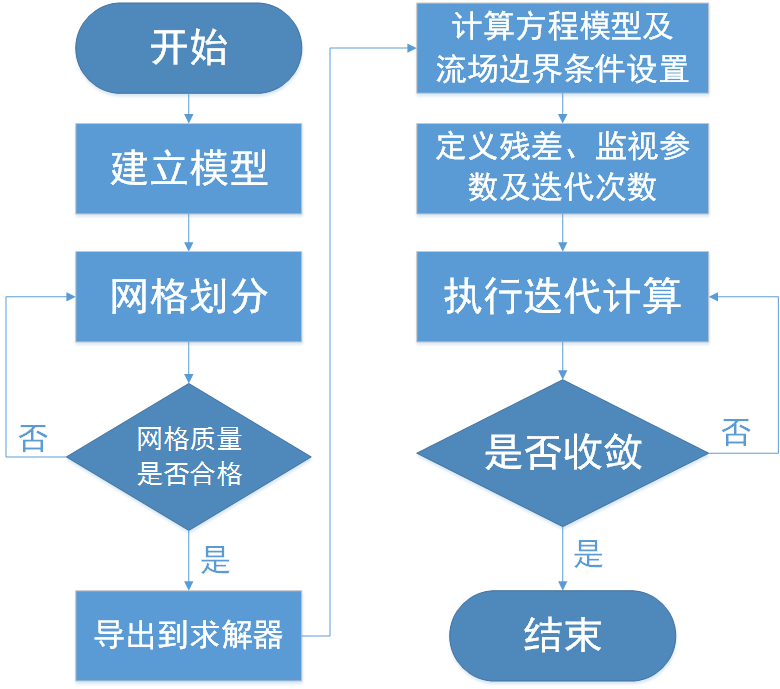
\includegraphics[width=0.65\linewidth]{liuchangmoniliuchengtu.png}
\caption{流场模拟流程图}
\label{fig:liuchangmoniliucheng}
\end{figure}
\subsection{导弹ICEM建模及基于Fluent的周围流场模拟}
为了研究导弹在高速飞行时周围流场的具体情况,可以利用已有的边界条件及计算方法,通过CFD软件对流场进行模拟,形象切量化地展现流场,并且由于流场的分析主要服务于对光传输的研究,因此弄清楚流场密度的分布尤其必要。为了在追求真实的同时减少计算量,本文利用ICEM建模软件建立了与实体尺寸类似的简易导弹模型,并且仅保留导弹的大致外形,去除弹载光学设备的结构,同时对导弹弹体进行了面型平滑处理,使导弹弹头呈球缺状半径为$0.5$m,弹体为圆柱弹身长$3.5$m,直径$1$m,尾翼为$1\text{m}\times1\text{m}\times0.1\text{m}$长方体减去一个厚度为$0.1$m的腰为$0.5$m的等腰三角形,如图\ref{fig:daodanmoxing}。

\begin{figure}[bhpt]
\centering
\subcaptionbox{三维导弹弹体模型\label{fig:daodanmoxing}}
{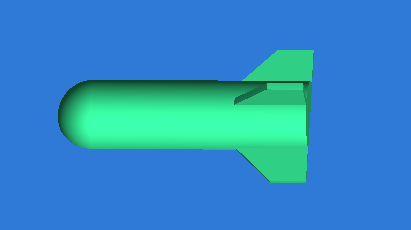
\includegraphics[width=0.45\linewidth]{daodanmoxing}}
\subcaptionbox{导弹轴面网格分布\label{fig:daodanwangge}}
{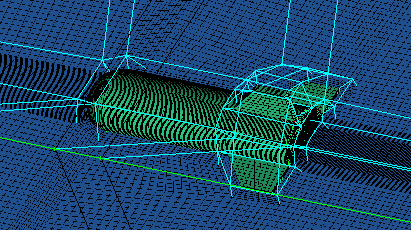
\includegraphics[width=.45\linewidth]{daodanwangge}}\\
\subcaptionbox{导弹弹体及流场截面网格分布\label{fig:daodanjubuwange}}
{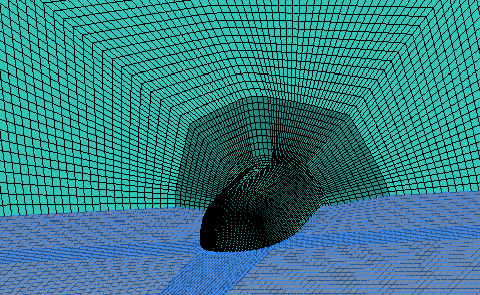
\includegraphics[width=0.45\linewidth]{daodanjubuwangge}}
\subcaptionbox{网格的质量评估\label{fig:wanggezhiliang}}
{\begin{minipage}{0.45\linewidth}
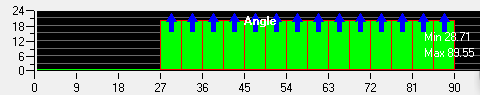
\includegraphics[width=\linewidth]{daodanwanggejiaodu}\\
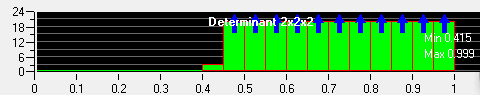
\includegraphics[width=\linewidth]{daodanwanggezhiliang}\\
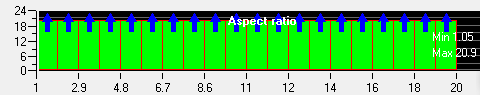
\includegraphics[width=\linewidth]{daodanwanggeniuqu}
\end{minipage}}
\caption{三维导弹模型及截面网格分布图}
\label{fig:daodan}
\end{figure}

建立完毕导弹的简易模型后,需要确定需要计算的区域,及外部流场的边界大小,本文在考虑外场边界时,令边界的下限取决于导弹飞行时对流场的影响距离,并且由于区域大小在一定程度上决定了计算量的多少,因此确定边界大小十分重要,为此本文选取长35m宽20高18m的长方体作为需要计算的流场区域。

由于理论上流场的计算并不能给出解析解,在引入亚格子模型后,可以得到流场的数值解,可以通过采用有限体积法及基于离散网格节点的梯度算法实现,因此需要对流场区域进行网格划分,网格的划分决定了计算的精度及准确度,决定了计算过程中结果是否收敛。本文将导弹周围的流场划分了230多万个计算网格,并且在导弹仅壁面处精细划分了20层加密层,如图\ref{fig:daodanwangge}、\ref{fig:daodanjubuwange},网格由弹体壁面向外辐射,且逐渐增大,既减增大了计算准确度,又减少了网格数量从而减少计算量。

由于飞行器结构具有不规则形,在计算时容易加大计算量,利用拓扑原理,将实体映射到规则的结构化六面体计算网格上是非常有效的方法,同时为了保证对应的网格具有可操作性,保证计算精度及结果的收敛情况,对划分的网格进行质量检查是必不可少的。
网格质量检查包括网格的行列式(Determinant)检查、角度(Angle)检查及横纵比(Aspect ratio)检查。
行列式检查是通过计算每一个六面体网格的雅可比行列式值,将行列式利用标准化的矩阵来表示单元的变形,值为1表示该网格是理想的六面体立方块,而值小于0则表示网格是具有负体积的反立方体,通常情况下行列式的值需要达到0.3以上才可以被大多数CFD求解器所接受。
角度检查则会对网格的每个单元的内角进行检测,$90\textdegree$表示两面是理想的正交面,角度越趋于$0\textdegree$则表示两个面夹角越小,对计算精度影响越大,Fluent中一般需要保证角度大于$18\textdegree$。
横纵比检查主要对比网格六面体每个面的长宽比值,值是1则表示该面是正方形,值越大表示面型越差,一般计算流体软件可以接受值100以下。

本文对导弹流场区域进行网格划分后,行列式质量检查全部达到0.4以上,网格总体质量令人满意,网格角度均大于$27\textdegree$,并且网格的单元面横纵比均小于20,网格质量检测结果如图\ref{fig:wanggezhiliang}。

导弹模型的前期处理完毕后,需要将完备的模型导入Fluent进行计算,由于
本文构建的导弹结构上具有对称性,因此为了减少计算量、提高效率,可以将导弹轴面设置成对称面,在计算完毕后以轴截面为对称面,z坐标取反后复制数据即可,此时可以将计算网格由初始值230万减少到115万个,大大提升了计算效率。

对于求解条件的设置,本文将导弹运行高度设置在海拔约1.5km的大气对流层,外界大气压为$85000$Pa,环境温度为$280$K,求解时基于离散方程,采用了第二章提出的与实验比较吻合的$k-\omega$SST修正模型计算方法,同时为了简化计算,根据相对性原理,将空气设为来流,导弹禁止不动,来流攻角为$0\textdegree$,模拟了导弹在低音速、音速、超音速等不同运行速度下的流场分布,如图\ref{fig:daodanliuchang}。

图\ref{fig:0.6daodanmidu}显示了0.6倍音速下,导弹弹体表面及流场轴截面的流场密度分布情况,可以发现在低音速情况下,飞行器周围并没有明显的剪切层及湍流的存在,流场密度分布约在0.9$\text{kg}/\text{m}^3$到1.3$\text{kg}/\text{m}^3$之间,导弹顶部气流压缩比较严重,密度较大,导弹头部与弹身交界处结构发生了较为明显的变化,流场密度最小,同时在尾翼处流场密度也比正常情况稍小。

\begin{figure}[bhtp]
\centering
\subcaptionbox{$u=0.6$Ma时密度分布,单位$(\text{kg}/\text{m}^3)$\label{fig:0.6daodanmidu}}{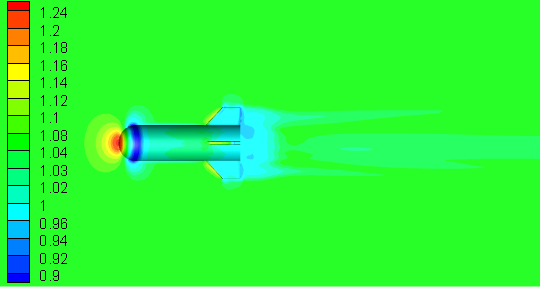
\includegraphics[width=0.45\linewidth]{0.6madaodanmidu.PNG}}
\subcaptionbox{$u=1$Ma时密度分布,单位$(\text{kg}/\text{m}^3)$\label{fig:1daodanmidu}}{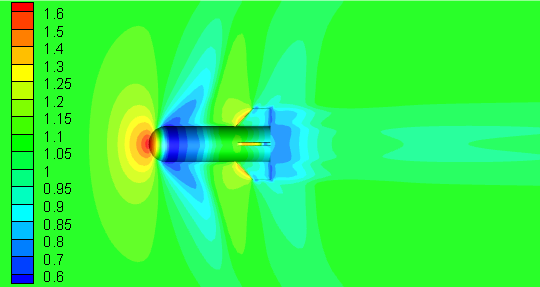
\includegraphics[width=0.45\linewidth]{1madaodanmidu.PNG}}\\
\subcaptionbox{$u=2$Ma时密度分布,单位$(\text{kg}/\text{m}^3)$\label{fig:2daodanmidu}}{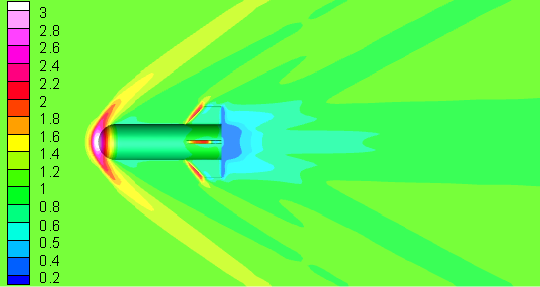
\includegraphics[width=0.45\linewidth]{2madaodanmidu.PNG}}
\subcaptionbox{$u=3$Ma时密度分布,单位$(\text{kg}/\text{m}^3)$\label{fig:3daodanmidu}}{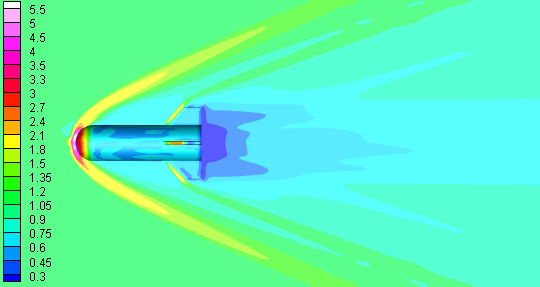
\includegraphics[width=0.45\linewidth]{3madaodanmidu.PNG}}
\caption{不同速度下导弹周围流场分布情况}
\label{fig:daodanliuchang}
\end{figure}

图\ref{fig:1daodanmidu}显示了1倍音速下,导弹弹体表面及流场轴截面的流场密度分布情况,可以看出导弹在以340m/s的速度运行时,密度场的分布情况与0.6倍音速下的密度有明显区别,在弹体及尾翼周围有截切层的存在,并且可以看到密度的不均匀分布,顶部由于与来流剧烈作用,空气发生压缩,密度较大,顶部密度在1.25$\text{kg}/\text{m}^3$到1.7$\text{kg}/\text{m}^3$之间分布,越靠近头部密度越大,而在弹身及尾翼这些外形结构有明显不同的周围,流场密度明显减小,越靠近壁面流场密度越小,往外呈辐射状分布。

图\ref{fig:2daodanmidu}显示了2倍音速下,导弹弹体表面及流场轴截面的流场密度分布情况,在图中可以明显看见剪切层的存在,在导弹顶部呈现压缩成碗底形的气流头罩,密度很大,在2$\text{kg}/\text{m}^3$到3.5$\text{kg}/\text{m}^3$之间,并且向外延伸出伞状剪切层,在尾翼出出现同样但是略微轻微的情况,尾后流场较为复杂,整体密度较小。

图\ref{fig:3daodanmidu}显示了三倍音速下,导弹弹体表面及流场轴截面的流场密度分布情况,在图中也与2倍音速下类似,可以明显看到周围的剪切层,但是相比于2倍音速下的流场情况,3Ma情况下的流场分布尤其是尾部分布更为复杂,通过对比可以看到外围的激波随着速度的增加,越来越靠近飞行器壁面且更薄,这与上一章中的分析是吻合的,飞行器对流场的影响整体后移,延伸距离更远,激波角度更小。

\begin{figure}[bhtp]
\centering
\subcaptionbox{1Ma速度下流场侧视图}{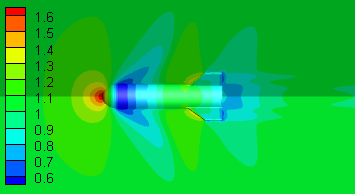
\includegraphics[width=0.47\linewidth]{1madaodancemianmidu.PNG}}
\subcaptionbox{2Ma速度下流场侧视图}{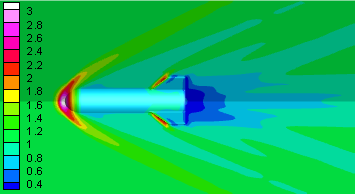
\includegraphics[width=0.47\linewidth]{2madaodancemianmidu.PNG}}
\caption{不同运行速度下导弹轴面及垂直截面的流场分布情况}
\label{fig:daodanceshi}
\end{figure}

图\ref{fig:daodanceshi}展示了运行速度分别为1Ma、2Ma下的导弹横截面以及垂直截面流场分布情况,通过两者对比可以发现,在2Ma运行速度下的截切层较为明显,在导弹头部周围形成的剪切层尤为明显,并且尾部流场也更加复杂,可以认为速度越快导弹周围的流场结构越复杂,那么对于光学成像、目标探测及制导的影响也就越大。

\subsection{机载凸台的ICEM模型建立及周围流场分析}
在对目标进行光学成像或追踪时,主要通过在飞行器侧面安装机载光学设备来获得目标信息,一般采用凸台或者凹窗结构,由于凸台光学设备可以大范围地收集观测目标信号,未来的应用将更加广泛,同时也会造成剧烈的流场波动,形成明显的截切层及湍流,周围会有大范围的密度梯度,可见示意图\ref{fig:tutailailiu}。
\begin{figure}[bthp]
\centering
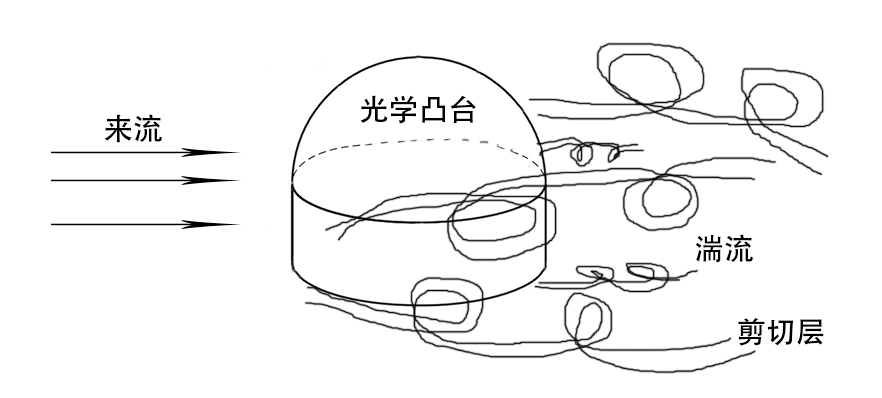
\includegraphics[width=0.8\linewidth]{tutailailiu.png}
\caption{光学凸台设备流场情况}
\label{fig:tutailailiu}
\end{figure}

由于机载凸台的尺寸相对于导弹较小,放在一起进行模拟计算时,由于网格尺度问题,很容易忽略机载凸台周围流场的细节,无法进一步进行研究分析,为此本文搭建了简易凸台模型,进行单独考虑,将凸台底部平面设置为无粘壁面,模拟导弹弹体表面。主要分析来流经过凸台后,凸台周围流场密度分布情况。

将简易凸台模型的下半部分定为圆柱体,半径$10$cm,高$10$cm,上半部分为半球,半径为$10$cm,在进行光信号接收时,凸台可以绕中轴360$\textdegree$旋转,探测范围很大,由于光学窗口主要位于半球处,在探究流场时,可以考虑离凸台底部10cm以上的流场区域。将外流场设置为$190\text{cm}\times200\text{cm}\times60\text{cm}$的长方体区域,机载光学凸台模型如图\ref{fig:tutaimoxing}。
\begin{figure}[bhpt]
\centering
\subcaptionbox{三维机载凸台模型\label{fig:tutaimoxing}}{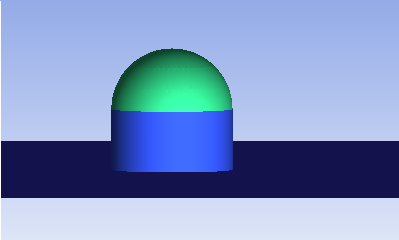
\includegraphics[width=0.45\linewidth]{tutaimoxing}}
\subcaptionbox{导凸台底面网格分布\label{fig:tutaiwangge}}{\centering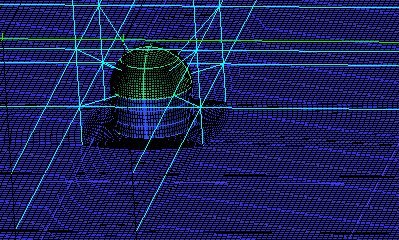
\includegraphics[width=.45\linewidth]{tutaiwangge}}
\subcaptionbox{凸台轴截面网格分布\label{fig:tutaijiemianwangge}}
{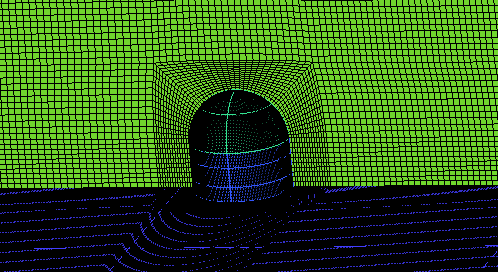
\includegraphics[width=.45\linewidth]{tutaijiemianwangge}}
\subcaptionbox{凸台整体网格的质量评估\label{fig:tutaiwanggezhiliang}}{\begin{minipage}[b]{0.45\linewidth}
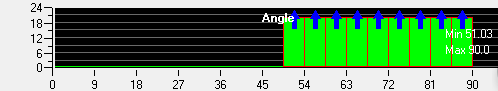
\includegraphics[width=\linewidth]{tutaiwanggejiaodu}\\
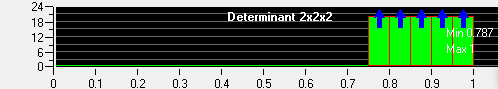
\includegraphics[width=\linewidth]{tutaiwanggezhengjiao}\\
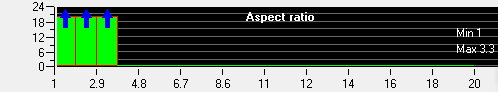
\includegraphics[width=\linewidth]{tutaiwanggeniuqu}
\end{minipage}}
\caption{三维凸台模型及截面网格分布图}
\label{fig:tutai}
\end{figure}

凸台的网格划分类似上一节导弹网格划分,将凸台周围的流场划分了约175万个计算网格,并且在导弹仅壁面处精细划分了17层宽为0.7mm的网络加密层,网格划分情况如图\ref{fig:tutaiwangge}、\ref{fig:tutaijiemianwangge},网格由凸台壁面向外辐射,外围网格保持均匀,便于数据导出及计算。
对凸台流场区域进行网格划分后,行列式质量检查全部达到0.75以上,网格总体质量非常好,网格角度均大于$50\textdegree$,表示计算网格扭曲度很小,并且网格的单元面横纵比均小于4,网格六面体比较接近理想正六面体,由于凸台外形简单,划分出的网格质量优于导弹的网格质量,导入流体计算软件后的计算精度更大,凸台的网格质量检测结果如图\ref{fig:wanggezhiliang}所示,至此凸台模型建立及网格划分处理完毕,满足计算要求,可以导入求解器进行模拟计算。

将凸台模型导入Fluent之后,检测完毕模型完整性及流场计算域的封闭性,设置模拟条件,可以参考上文导弹参数设置,将运行高度设置在海拔约1.5km的大气对流层,外界大气压为$85000$Pa,环境温度为$280$K,采用Menter提出的$k-\omega$二方程SST模型结合J-B修正模型。

同样为了简化计算,根据相对性原理,将空气设为来流,凸台禁止不动,来流攻角为$0\textdegree$,凸台底部应设置为符合导弹表面情况的的无粘壁面。由于考虑到光学窗口位置,在凸台半腰处设置一个观察平面,方便观测凸台周围的流场情况,本文模拟了在0.6倍音速、1倍音速及2倍音速三种不同运行速度下,凸台周围的流场分布,如图\ref{fig:tutailiuchang}。

图\ref{fig:0.6tutaimidu}显示了0.6倍音速下,观测截面及凸台表面的流场密度分布情况,可以发现在低音速情况下,物体周围并没有明显的剪切层存在,流场密度分布约在0.75$\text{kg}/\text{m}^3$到1.$\text{kg}/\text{m}^3$之间,凸台与来流直接接触的地方气流存在压缩及反弹情况,密度较大,凸台外侧靠近壁面部分流场密度有波动,且在凸台轴界面部分区域流场密度最小,在0.7$\text{kg}/\text{m}^3$到0.9$\text{kg}/\text{m}^3$之间。

图\ref{fig:1tutaimidu}显示了1倍音速下,观测截面及凸台表面的流场密度分布情况,可以看运行速度为340m/s时,密度场的分布情况与0.6倍音速下的密度区别较大,流场波动范围更加广,凸台周围有截切层的存在,可以看到密度的不均匀分布及不明显的分层,凸台前沿与来流剧烈作用,空气发生压缩,密度较大,接触面外侧流场密度约在1.3$\text{kg}/\text{m}^3$到1.7$\text{kg}/\text{m}^3$之间分布,并且空气有反弹情况出现,尾部流场扩散明显,影响范围较广,但是波动并不是很明显。

\begin{figure}[bhtp]
\centering
\subcaptionbox{$u=0.6$Ma时密度分布,单位$(\text{kg}/\text{m}^3)$\label{fig:0.6tutaimidu}}{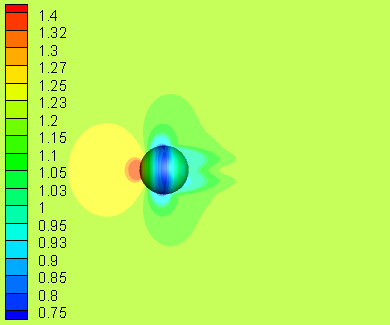
\includegraphics[width=0.45\linewidth]{0.6matutaimidu1.PNG}}
\subcaptionbox{$u=1$Ma时密度分布,单位$(\text{kg}/\text{m}^3)$\label{fig:1tutaimidu}}{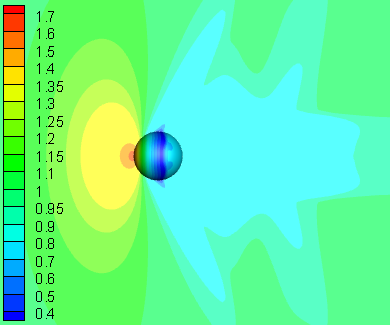
\includegraphics[width=0.45\linewidth]{1matutaimidu1.PNG}}\\
\subcaptionbox{$u=2$Ma时密度分布,单位$(\text{kg}/\text{m}^3)$\label{fig:2tutaimidu}}{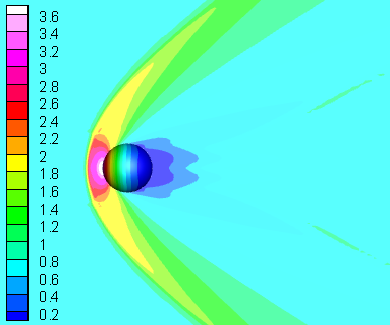
\includegraphics[width=0.45\linewidth]{2matutaimidu1.PNG}}
\subcaptionbox{$u=2$Ma时温度度分布,单位$(\text{K})$\label{fig:2tutaiwendu}}{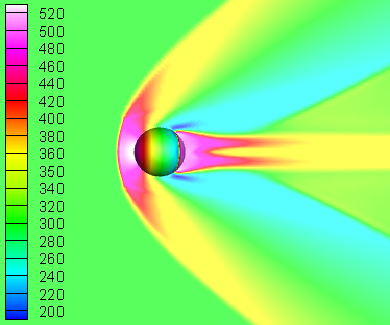
\includegraphics[width=0.45\linewidth]{2matutaiwendu1.PNG}}
\caption{不同速度下凸台周围流场分布情况}
\label{fig:tutailiuchang}
\end{figure}

图\ref{fig:2tutaimidu}显示了2倍音速下,观测截面及凸台表面的流场密度分布情况,在图中能够明显看见剪切层的存在,在导弹顶部呈现压缩成蘑菇形的气流头罩,密度很大,在2$\text{kg}/\text{m}^3$到4$\text{kg}/\text{m}^3$之间,并且向外延伸出抛物面型剪切层,图中可以明显看出凸台近壁面流场分层情况,由前方过度到中轴面再到凸台后部,密度由大到小呈现梯度递减。在凸台后方的近场密度分布也有明显分层且不规则分布,剪切层向中心靠拢,与实验数据较为吻合。

图\ref{fig:2tutaiwendu}显示了2Ma时凸台周围流场温度分布情况,温度分布与密度分布情况比较符合,同时更加详细地显示了凸台后方近场流场分布,外侧有低温地带,中心温度较高并且由内向外呈梯度分布。

通过对光学机载凸台周围流场的数值模拟,可以更加清晰的描述光学窗口的处流场结构,为接下来的光传输特性的数值计算提供流场物理参数的数据支撑。
\section{本章小结}
本章对求解流场分布所需的定解条件作了相应说明及设置,推导了利用隐式迭代法求解离散方程的过程,并且对模拟的前期面型、网格等进行了优化,最后采用SST$k-\omega$二方程修正模型,基于有限体积法数值模拟了低音速、音速、超音速等不同运行速度下导弹及机载光学凸台周围的流场情况,并详细分析了流场模拟结果。

